\documentclass[11pt]{article}
\usepackage[margin=18mm,headheight=22pt]{geometry}
\usepackage{amsmath}
\usepackage{fontspec}
\usepackage{unicode-math}
\setmainfont{NewCM10}[Extension=.otf,UprightFont=*-Book,BoldFont=*-Bold,ItalicFont=*-BookItalic,BoldItalicFont=*-BoldItalic]
\setsansfont{NewCMSans10}[Extension=.otf,UprightFont=*-Book,BoldFont=*-Bold,ItalicFont=*-BookOblique,BoldItalicFont=*-BoldOblique]
\setmathfont{NewCMMath-Book.otf}
\usepackage{xcolor}
\definecolor{FAUblue}{HTML}{04316A}
\definecolor{Paperblue}{HTML}{EEF2F7}
\definecolor{EEIgold}{HTML}{CC9C42}
\usepackage{etoolbox,enumitem,booktabs,tabularx,array,needspace,microtype}
\usepackage[most]{tcolorbox}
\usepackage{titlesec,fancyhdr}
\usepackage[hidelinks]{hyperref}
\usepackage{draftwatermark}
\SetWatermarkText{Made by Thanate Amornjiraporn (Focus)}
\SetWatermarkColor{black!7}\SetWatermarkFontSize{30pt}\SetWatermarkAngle{45}
\setlength{\parindent}{0pt}
\setlength{\parskip}{5pt}
\setlist{itemsep=2pt,topsep=3pt,leftmargin=1.6em,beginpenalty=10000,endpenalty=10000}
\raggedbottom
\clubpenalty=10000 \widowpenalty=10000 \displaywidowpenalty=10000 \interlinepenalty=10000
\setcounter{secnumdepth}{0}
\setcounter{tocdepth}{1}
\pagestyle{fancy}\fancyhf{}
\fancyhead[L]{\small\sffamily\color{FAUblue} From Fundamentals to AI Apocalypse · APDR · Chapter 6}
\fancyhead[R]{\small\sffamily Python Basics, Branching, and Iteration}
\fancyfoot[C]{\small\thepage}
\titleformat{\section}{\Large\bfseries\sffamily\color{FAUblue}}{}{0pt}{}
\titleformat{\subsection}{\large\bfseries\sffamily\color{FAUblue}}{}{0pt}{}
\titlespacing*{\section}{0pt}{16pt}{6pt}
\preto\section{\Needspace{8\baselineskip}}
\preto\subsection{\Needspace{6\baselineskip}}
\newtcolorbox{equationcard}[1]{colback=Paperblue,colframe=Paperblue,boxrule=0pt,arc=0pt,left=10pt,right=10pt,top=6pt,bottom=6pt,title={#1},fonttitle=\small\bfseries\sffamily,coltitle=FAUblue,before skip=8pt,after skip=8pt}
\newtcolorbox{workedbox}[1]{colback=white,colframe=EEIgold,boxrule=0pt,leftrule=3pt,arc=0pt,left=10pt,top=4pt,bottom=4pt,title={#1},fonttitle=\small\bfseries\sffamily,coltitle=FAUblue,attach title to upper={\par},before skip=8pt,after skip=8pt}
\newtcolorbox{recallbox}[1]{colback=white,colframe=FAUblue,boxrule=0pt,leftrule=3pt,arc=0pt,left=10pt,top=4pt,bottom=4pt,title={#1},fonttitle=\small\bfseries\sffamily,coltitle=FAUblue,attach title to upper={\par},before skip=8pt,after skip=8pt}
\usepackage{environ}
\newsavebox\measurebox
% Typeset the section once invisibly to measure it; start a new page if it will not fit in what is left.
\makeatletter
\newif\ifkeep@measuring
\NewEnviron{keepsection}{%
  \ifkeep@measuring \BODY \else
    \edef\keep@sec{\the\value{section}}\edef\keep@sub{\the\value{subsection}}%
    \setbox\measurebox\vbox{\hsize\linewidth\keep@measuringtrue\def\Needspace##1{}\BODY}%
    \setcounter{section}{\keep@sec}\setcounter{subsection}{\keep@sub}%
    \dimen2=\ht\measurebox \advance\dimen2\dp\measurebox
    \dimen@=\textheight
    \ifdim\pagegoal<\maxdimen
      \dimen@=\pagegoal \advance\dimen@-\pagetotal
      \ifdim\dimen2>\dimen@ \clearpage \dimen@=\textheight \fi
    \fi
    % if it fits, nothing inside may force an early break
    \ifdim\dimen2>\dimen@ \BODY \else \begingroup\def\Needspace##1{}\BODY\endgroup \fi
  \fi}
\makeatother
\newtcolorbox{notebox}{colback=Paperblue,colframe=Paperblue,boxrule=0pt,arc=0pt,left=8pt,right=8pt,top=4pt,bottom=4pt,before skip=6pt,after skip=6pt}
\newtcolorbox{plainbox}{colback=white,colframe=FAUblue,boxrule=0pt,leftrule=3pt,arc=0pt,left=10pt,right=8pt,top=4pt,bottom=4pt,before skip=6pt,after skip=8pt}
\usetikzlibrary{arrows.meta}
\title{\sffamily\bfseries\color{FAUblue}Python Basics, Branching, and Iteration}
\author{Algorithms, Programming, and Data Representation \ensuremath{\cdot} Module 23131 \ensuremath{\cdot} Chapter 6\\[2pt]\small From Fundamentals to AI Apocalypse · personal study guide}
\date{}
\begin{document}
\maketitle
\begingroup\footnotesize\setlength{\parskip}{0pt}\tableofcontents\endgroup
\clearpage

\Needspace{9\baselineskip}
{\large This chapter builds the first working Python: values and their types, operators, names bound to values, strings, printing and reading input, and the two control-flow tools every program needs, choosing a branch and repeating a block.}


\begin{keepsection}
\Needspace{13\baselineskip}
\section{Start from memory}

\Needspace{10\baselineskip}
Try each question first. Mark it sure, unsure, or guessed.

\Needspace{8\baselineskip}
\begin{enumerate}
\item What is the type of the value of \texttt{7 / 7} in Python?
\item What does \texttt{"abc"[-1]} evaluate to?
\item What is the difference between \texttt{=} and \texttt{==}?
\item Which numbers does \texttt{range(5)} produce?
\item What does \texttt{break} do inside two nested loops?
\end{enumerate}

\nopagebreak[4]{\small\itshape Answers: see “Start from memory” under Answers at the end.}
\end{keepsection}

\begin{keepsection}
\Needspace{20\baselineskip}
\section{How to use this guide}

\Needspace{17\baselineskip}
Read a section, close it, and type its examples into a Python shell from memory before you check them. The lecture’s own advice applies to every line here: if you are unsure what a command does, try it in the console.

\Needspace{13\baselineskip}
\begin{enumerate}
\item \textbf{Day 0:} Try the cold start, then study §6.1–6.4; solve practice 1, 2, 3, 5, 12.
\item \textbf{Day 1:} Rebuild §6.1–6.4 from memory, then study §6.5–6.7; solve practice 6, 8, 9, 15, 18, 19.
\item \textbf{Day 3:} Rebuild §6.5–6.7 from memory, then study §6.8–6.10 and trace every loop on paper; solve practice 4, 7, 11, 13, 14, 17.
\item \textbf{About day 7:} Do the derivation list cold, then practice 10, 16, 20–24 without notes.
\item \textbf{About day 14:} Work both exam problems in 20 minutes each; answer the “Explain it” questions aloud.
\item \textbf{Before the exam:} Tick only the self-check skills you can show cold; revisit the sections named in the answers you missed.
\end{enumerate}

\begin{notebox}\textbf{When stuck:} make a trace table. Write one column per variable and one row per line executed, and fill it in line by line. Most loop and branch questions are answered by the last row.\end{notebox}
\end{keepsection}

\begin{keepsection}
\Needspace{24\baselineskip}
\section{How the chapter fits together}

\Needspace{21\baselineskip}
Values with types come first, because operators and comparisons depend on the type. Names hold values, strings are a sequence type, and input and output connect a program to its user. Branching and loops then decide which lines run and how often.

\Needspace{8\baselineskip}
\textbf{Measure} \ensuremath{\cdot} values and types

\Needspace{6\baselineskip}
\begin{itemize}
\item \Needspace{4\baselineskip}
\textbf{Objects and types} \hfill{\small\color{FAUblue}§6.1}

\Needspace{5\baselineskip}
\texttt{int \ensuremath{\cdot} float \ensuremath{\cdot} bool \ensuremath{\cdot} NoneType}

Rests on: nothing earlier; every value in a program has a type that fixes what you can do with it.
\item \Needspace{4\baselineskip}
\textbf{Expressions and operators} \hfill{\small\color{FAUblue}§6.2}

\Needspace{4\baselineskip}
\texttt{i // j \ensuremath{\cdot} i \% j \ensuremath{\cdot} i ** j}

Rests on: types, because the operand types decide the result type.
\end{itemize}

\Needspace{13\baselineskip}
\textbf{Define} \ensuremath{\cdot} names, text and comparison

\Needspace{11\baselineskip}
\begin{itemize}
\item \Needspace{4\baselineskip}
\textbf{Assignment} \hfill{\small\color{FAUblue}§6.3}

\Needspace{5\baselineskip}
\texttt{name = expression}

Rests on: expressions, because the right side is evaluated to a value before the name is bound.
\item \Needspace{4\baselineskip}
\textbf{Strings} \hfill{\small\color{FAUblue}§6.4}

\Needspace{4\baselineskip}
\texttt{s[start:stop:step]}

Rests on: types and names; a string is an immutable sequence you reach through a name.
\item \Needspace{4\baselineskip}
\textbf{Output and input} \hfill{\small\color{FAUblue}§6.5}

\Needspace{4\baselineskip}
\texttt{int(input(…))}

Rests on: strings and casting, because \texttt{input} always returns a string.
\item \Needspace{4\baselineskip}
\textbf{Comparison and logic} \hfill{\small\color{FAUblue}§6.6}

\Needspace{4\baselineskip}
\texttt{== != \ensuremath{<} \ensuremath{>} and or not}

Rests on: expressions; comparisons are expressions whose value is a Boolean.
\end{itemize}

\Needspace{12\baselineskip}
\textbf{Derive} \ensuremath{\cdot} control flow

\Needspace{10\baselineskip}
\begin{itemize}
\item \Needspace{4\baselineskip}
\textbf{Branching} \hfill{\small\color{FAUblue}§6.7}

\Needspace{4\baselineskip}
\texttt{if \ensuremath{\cdot} elif \ensuremath{\cdot} else}

Rests on: comparisons, because each condition is a Boolean expression.
\item \Needspace{4\baselineskip}
\textbf{while and for} \hfill{\small\color{FAUblue}§6.8}

\Needspace{4\baselineskip}
\texttt{range(start, stop, step)}

Rests on: conditions and rebinding; a loop repeats while a condition holds or once per value.
\item \Needspace{4\baselineskip}
\textbf{break and continue} \hfill{\small\color{FAUblue}§6.9}

\Needspace{4\baselineskip}
\texttt{break \ensuremath{\cdot} continue}

Rests on: loops and branches; a jump is almost always inside an \texttt{if} inside a loop.
\item \Needspace{4\baselineskip}
\textbf{Choosing a loop} \hfill{\small\color{FAUblue}§6.10}

\Needspace{4\baselineskip}
\texttt{for char in s}

Rests on: both loop kinds and on strings as sequences.
\end{itemize}

\Needspace{16\baselineskip}
\Needspace{10\baselineskip}
\begin{center}\small\begin{tabularx}{\linewidth}{>{\raggedright\arraybackslash}X>{\raggedright\arraybackslash}X}\toprule
\textbf{Question} & \textbf{Tool} \\ \midrule
What value and type does this expression have? & Operand types and precedence (§6.1–6.2) \\
What does this name hold after these lines? & A trace table of assignments (§6.3) \\
Which characters does this index or slice give? & Write the indices under the string (§6.4) \\
Which lines run? & Evaluate each condition in order (§6.6–6.7) \\
How often does the body run, and what is left? & Trace the loop variable row by row (§6.8–6.9) \\
Which loop should I write? & Known count \ensuremath{\to} \texttt{for}; stop on a condition \ensuremath{\to} \texttt{while} (§6.10) \\
\bottomrule\end{tabularx}\end{center}
\end{keepsection}

\begin{keepsection}
\Needspace{12\baselineskip}
\section{6.1 Programs, Python, objects and types}

\Needspace{9\baselineskip}
Before any branching or looping, you need to know what a program is made of and what kinds of values it handles.

\Needspace{13\baselineskip}
\begin{plainbox}\textbf{In plain words:} a \textbf{program} is a list of definitions and commands written as text, the \textbf{source code}. The processor cannot read that text; it only runs its own machine instructions. A \textbf{compiler} translates the whole text into machine code first, while an \textbf{interpreter}, like Python’s, reads and runs it line by line. Every value the program touches is an \textbf{object} with a \textbf{type}, and the type decides what you may do with it, just as a car can drive but cannot swim.\end{plainbox}

\begin{equationcard}{The scalar types}
\[ \begin{gathered} \texttt{int}\, \cdot \, \texttt{float}\, \cdot \, \texttt{bool}\, \cdot \, \texttt{NoneType} \\ \texttt{type(5)}\, \to \, \texttt{int} \\ \texttt{type(3.0)}\, \to \, \texttt{float} \end{gathered} \]
{\small \emph{Read it as: “the type of 5 is int, the type of 3.0 is float”.}\par  \texttt{int} holds whole numbers, \texttt{float} real numbers, \texttt{bool} the two values \texttt{True} and \texttt{False}, and \texttt{NoneType} the single value \texttt{None}.}
\end{equationcard}

\begin{equationcard}{Casting}
\[ \begin{gathered} \texttt{float(3)}\, \to \, \texttt{3.0} \\ \texttt{int(3.9)}\, \to \, \texttt{3} \end{gathered} \]
{\small \emph{Read it as: “float of 3 is 3.0; int of 3.9 is 3”.}\par  Converting a value to another type is called casting. \texttt{int} of a float cuts off the fractional part; it does not round.}
\end{equationcard}

\Needspace{8\baselineskip}
Python is an interpreted language: you can type commands into a shell one at a time, store them in a file that the interpreter reads, or run them in a notebook. The lecture uses Python as one example of an imperative language; the ideas in this chapter carry over to the others. Functional languages such as Haskell work differently and are not part of the course.

\Needspace{7\baselineskip}
The lecture separates two kinds of line. A \textbf{definition} is evaluated: Python works out what it means. A \textbf{command} (or statement) is executed: it tells the interpreter to do something.

\Needspace{12\baselineskip}
Objects are either \textbf{scalar}, meaning they cannot be split into parts (a number, a Boolean), or \textbf{non-scalar}, meaning they have an internal structure you can reach into. A string, met in §6.4, is the first non-scalar type.

\begin{workedbox}{Worked example \ensuremath{\cdot} types and casts}
\Needspace{9\baselineskip}
\begin{enumerate}
\item \texttt{type(True)} is \texttt{bool}: \texttt{True} is a Boolean value, not a string.
\item \texttt{float(7)} is \texttt{7.0}: same number, now a float.
\item \texttt{int(-3.9)} is \texttt{-3}: the fractional part is cut off towards zero, so a negative number moves up, not down.
\item Check: each result has the type named by the cast, and no value changed by more than its fractional part.
\end{enumerate}
\end{workedbox}

\Needspace{5\baselineskip}
\begin{notebox}\textbf{Trap:} \texttt{int(3.9)} is 3, not 4. Casting truncates; use \texttt{round} when you mean rounding.\end{notebox}

\Needspace{12\baselineskip}
\begin{notebox}\textbf{Near miss:} \texttt{"5"} looks like the number 5, but the quotes make it a string; \texttt{type("5")} is \texttt{str}. Cast it with \texttt{int("5")} before doing arithmetic.\end{notebox}

\begin{recallbox}{Recall check \ensuremath{\cdot} answer without looking}
\Needspace{5\baselineskip}
\begin{enumerate}
\item Why does a computer need a compiler or an interpreter to run Python source code?
\item Name the four scalar types and one value of each.
\item What is \texttt{int(-2.5)}?
\end{enumerate}

\nopagebreak[4]{\small\itshape Answers: see “6.1 Programs, Python, objects and types” under Answers at the end.}
\end{recallbox}
\end{keepsection}

\begin{keepsection}
\Needspace{10\baselineskip}
\section{6.2 Expressions and operators}

\Needspace{7\baselineskip}
Objects become useful when operators combine them into expressions; the operand types decide the type of the answer.

\Needspace{11\baselineskip}
\begin{plainbox}\textbf{In plain words:} an \textbf{expression} joins objects with \textbf{operators}, like \texttt{3 + 2}, and Python works it out to a single \textbf{value}. That value has a type too. When several operators meet, \textbf{precedence} says which goes first, the way multiplication beats addition in arithmetic, and brackets override it.\end{plainbox}

\begin{equationcard}{Arithmetic operators}
\[ \begin{gathered} \texttt{i + j}\, \cdot \, \texttt{i - j}\, \cdot \, \texttt{i * j}:\, \text{int}\, \text{if}\, \text{both}\, \text{are}\, \text{int},\, \text{else}\, \text{float} \\ \texttt{i / j}:\, \text{always}\, \mathrm{a}\, \text{float} \\ \texttt{i ** j}\, =\, {i}^{{j}} \end{gathered} \]
{\small \emph{Read it as: “sum, difference and product are int only when both operands are int; division always gives a float; i to the power j”.}\par  \texttt{6 / 3} is \texttt{2.0}, not 2.}
\end{equationcard}

\begin{equationcard}{Floor division and remainder}
\[ \begin{gathered} \texttt{i // j}\, =\, ⌊\dfrac{{i}}{{j}}⌋ \\ \texttt{i \% j}\, =\, {i}\, -\, {j}\, \cdot \, (\texttt{i // j}) \end{gathered} \]
{\small \emph{Read it as: “i floor-divided by j is i over j rounded down; i mod j is what is left after taking j that many times”.}\par  For two ints, \texttt{7 // 2} is 3 and \texttt{7 \% 2} is 1. With a float operand the quotient is a float: \texttt{7.0 // 2} is \texttt{3.0}.}
\end{equationcard}

\Needspace{14\baselineskip}
\begin{center}
\begin{minipage}[t]{0.950\linewidth}\centering
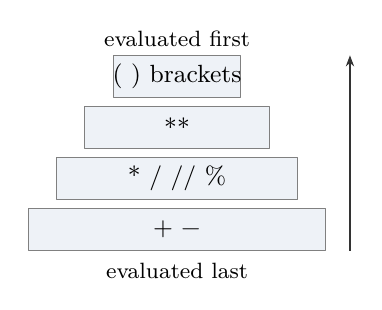
\begin{tikzpicture}[line join=round]
\node[,inner sep=1pt,font=\footnotesize] at (2.340,-0.216) {evaluated first};
\filldraw[draw=black!50,fill=Paperblue] (1.530,-0.432) rectangle (3.150,-0.972);
\node[,inner sep=1pt,font=\small] at (2.340,-0.702) {( ) brackets};
\filldraw[draw=black!50,fill=Paperblue] (1.170,-1.080) rectangle (3.510,-1.620);
\node[,inner sep=1pt,font=\small] at (2.340,-1.350) {**};
\filldraw[draw=black!50,fill=Paperblue] (0.810,-1.728) rectangle (3.870,-2.268);
\node[,inner sep=1pt,font=\small] at (2.340,-1.998) {* / // \%};
\filldraw[draw=black!50,fill=Paperblue] (0.450,-2.376) rectangle (4.230,-2.916);
\node[,inner sep=1pt,font=\small] at (2.340,-2.646) {+ \ensuremath{-}};
\draw[-{Stealth[length=4pt]},black!80] (4.536,-2.916) -- (4.536,-0.432);
\node[,inner sep=1pt,font=\footnotesize] at (2.340,-3.168) {evaluated last};
\end{tikzpicture}\par\smallskip{\small\raggedright \textbf{Precedence.} A higher row is evaluated before a lower one; operators in the same row go left to right, except \texttt{**}.\par}\end{minipage}
\end{center}

\Needspace{9\baselineskip}
The interactive shell shows the value of a bare expression: typing \texttt{3+2} prints \texttt{Out[11]: 5} in the lecture’s IPython console. A program that should show something to a user calls \texttt{print} instead (§6.5).

\Needspace{13\baselineskip}
The general shape is \texttt{\ensuremath{<}object\ensuremath{>} \ensuremath{<}operator\ensuremath{>} \ensuremath{<}object\ensuremath{>}}. Without brackets Python applies \texttt{**} first, then the multiplicative operators, then \texttt{+} and \texttt{-}. The lecture lists \texttt{*} and \texttt{/} on separate rows; in Python they share one row with \texttt{//} and \texttt{\%} and are evaluated left to right, so \texttt{8 / 2 * 4} is \texttt{16.0} (see the slips list). \texttt{+} and \texttt{-} also go left to right: \texttt{10 - 4 - 3} is 3.

\begin{workedbox}{Worked example \ensuremath{\cdot} evaluate 2 + 3 * 4 ** 2 // 5}
\Needspace{8\baselineskip}
\begin{enumerate}
\item Power first: \texttt{4 ** 2} is 16, giving \texttt{2 + 3 * 16 // 5}.
\item \texttt{*} and \texttt{//} share a row, so left to right: \texttt{3 * 16} is 48, then \texttt{48 // 5} is 9 (48 ÷ 5 = 9.6, rounded down).
\item Last the addition: \texttt{2 + 9} is 11, an \texttt{int} because every operand was an int.
\item Check: no \texttt{/} appeared, so no float can appear; 11 is an int.
\end{enumerate}
\end{workedbox}

\Needspace{6\baselineskip}
\begin{notebox}\textbf{Trap:} \texttt{//} rounds down, not towards zero. \texttt{-7 // 2} is \texttt{-4}, and then \texttt{-7 \% 2} is 1 so that the identity above still holds.\end{notebox}

\Needspace{5\baselineskip}
\begin{notebox}\textbf{Near miss:} \texttt{6 / 3} divides evenly, so it is tempting to expect the int 2, but \texttt{/} always returns a float: the value is \texttt{2.0}. Write \texttt{6 // 3} for the int.\end{notebox}

\Needspace{9\baselineskip}
\begin{recallbox}{Recall check \ensuremath{\cdot} answer without looking}
\Needspace{5\baselineskip}
\begin{enumerate}
\item What are the value and type of \texttt{7 // 2} and of \texttt{7 / 2}?
\item Evaluate \texttt{2 ** 3 ** 2} and say why.
\item What is \texttt{17 \% 5}?
\end{enumerate}

\nopagebreak[4]{\small\itshape Answers: see “6.2 Expressions and operators” under Answers at the end.}
\end{recallbox}
\end{keepsection}

\begin{keepsection}
\Needspace{11\baselineskip}
\section{6.3 Variables and assignment}

\Needspace{8\baselineskip}
Naming a value lets you reuse it and change the program in one place; the equals sign does this, but it does not mean what it means in maths.

\Needspace{12\baselineskip}
\begin{plainbox}\textbf{In plain words:} an \textbf{assignment} sticks a name label on a value stored in memory, the way a \textbf{variable} name points at a number. Python first works out the expression on the right, then binds the name on the left to the result. You can move the label to a new value later (\textbf{rebinding}); anything worked out earlier from the old value stays as it was.\end{plainbox}

\begin{equationcard}{Assignment}
\[ \begin{gathered} \texttt{name = expression} \\ \texttt{radius += 1}\, \text{means}\, \texttt{radius = radius + 1} \end{gathered} \]
{\small \emph{Read it as: “evaluate the expression, then bind the name to that value”.}\par  The name is on the left, the expression on the right. \texttt{radius = radius + 1} is not an equation to solve: it reads the old value, adds 1, and rebinds.}
\end{equationcard}

\Needspace{14\baselineskip}
\begin{center}
\begin{minipage}[t]{0.950\linewidth}\centering
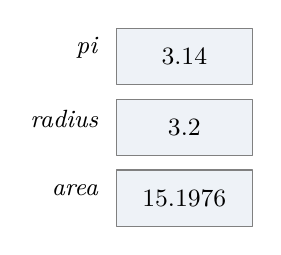
\begin{tikzpicture}[line join=round]
\node[anchor=east,inner sep=1pt,font=\small] at (1.800,-0.432) {\textit{pi}};
\draw[black!50,fill=Paperblue] (1.980,-0.180) rectangle (3.708,-0.900);
\node[,inner sep=1pt,font=\small] at (2.844,-0.540) {3.14};
\node[anchor=east,inner sep=1pt,font=\small] at (1.800,-1.332) {\textit{radius}};
\draw[black!50,fill=Paperblue] (1.980,-1.080) rectangle (3.708,-1.800);
\node[,inner sep=1pt,font=\small] at (2.844,-1.440) {3.2};
\node[anchor=east,inner sep=1pt,font=\small] at (1.800,-2.232) {\textit{area}};
\draw[black!50,fill=Paperblue] (1.980,-1.980) rectangle (3.708,-2.700);
\node[,inner sep=1pt,font=\small] at (2.844,-2.340) {15.1976};
\end{tikzpicture}\par\smallskip{\small\raggedright \textbf{After the lecture’s four lines.} \texttt{radius} now holds 3.2, but \texttt{area} still holds the value worked out from 2.2: nothing recalculates it.\par}\end{minipage}
\end{center}

\Needspace{9\baselineskip}
Retrieve a value by typing its name: after \texttt{pi = 3.14159}, the name \texttt{pi} evaluates to 3.14159. Names make code easier to read and to change: \texttt{area = pi*(radius**2)} says what it computes, and changing \texttt{radius} in one place changes every line that uses it when that line next runs.

\Needspace{13\baselineskip}
A name may contain letters, digits and underscores but may not start with a digit, may not contain a dot, and may not be a keyword such as \texttt{if} or \texttt{for}; the slide’s \texttt{pi\_approx. = 22/7} is a syntax error for that reason (see the slips list). After a rebinding the old value may still sit in memory, but the program has lost its handle on it.

\begin{workedbox}{Worked example \ensuremath{\cdot} trace the lecture’s lines}
\Needspace{8\baselineskip}
\begin{enumerate}
\item \texttt{pi = 3.14} binds \texttt{pi} to 3.14; \texttt{radius = 2.2} binds \texttt{radius} to 2.2.
\item \texttt{area = pi*(radius**2)} evaluates 3.14 \ensuremath{\cdot} 4.84 = 15.1976 and binds \texttt{area} to it.
\item \texttt{radius = radius+1} reads 2.2, adds 1 and rebinds \texttt{radius} to 3.2.
\item Check: \texttt{area} is still 15.1976. To update it you must run the area line again. (Python prints 15.197600000000003; the tail is float rounding, Chapter 4.)
\end{enumerate}
\end{workedbox}

\Needspace{6\baselineskip}
\begin{notebox}\textbf{Trap:} a variable is not a formula. Changing \texttt{radius} does not change \texttt{area}; only re-running the assignment does.\end{notebox}

\Needspace{12\baselineskip}
\begin{notebox}\textbf{Near miss:} \texttt{x + 1 = 5} reads like an equation with the answer \texttt{x = 4}, but it is a syntax error: the left side of \texttt{=} must be a name, not an expression. Python never solves for \textit{x}.\end{notebox}

\begin{recallbox}{Recall check \ensuremath{\cdot} answer without looking}
\Needspace{4\baselineskip}
\begin{enumerate}
\item In \texttt{count = count + 1}, which side is evaluated first, and what happens next?
\item Give two reasons to name values instead of writing the numbers each time.
\end{enumerate}

\nopagebreak[4]{\small\itshape Answers: see “6.3 Variables and assignment” under Answers at the end.}
\end{recallbox}
\end{keepsection}

\begin{keepsection}
\Needspace{12\baselineskip}
\section{6.4 Strings}

\Needspace{9\baselineskip}
Text is the first non-scalar type: a string has parts you can index and slice, which loops in §6.10 will walk through.

\Needspace{14\baselineskip}
\begin{plainbox}\textbf{In plain words:} a \textbf{string} is a row of characters (letters, digits, spaces, symbols) written in single or double quotes. Each character has a position number, its \textbf{index}, starting at 0 from the left and at \ensuremath{-}1 from the right. A \textbf{slice} cuts out a piece by giving where to start, where to stop and how big a step to take. Strings are \textbf{immutable}: you cannot change a character in place, only build a new string.\end{plainbox}

\begin{equationcard}{String operations}
\[ \begin{gathered} \texttt{"ab" + "cd"}\, \to \, \texttt{"abcd"} \\ \texttt{"ab" * 3}\, \to \, \texttt{"ababab"} \\ \texttt{len("abc")}\, \to \, \texttt{3} \end{gathered} \]
{\small \emph{Read it as: “plus joins strings, times repeats a string, len counts its characters”.}\par  Joining is called concatenation. \texttt{+} does not insert a space: \texttt{"hello there" + "Joe"} is \texttt{"hello thereJoe"}. \texttt{*} binds before \texttt{+} here too: with \texttt{name = "Joe"}, \texttt{"hi " + name * 3} is \texttt{"hi JoeJoeJoe"}.}
\end{equationcard}

\begin{equationcard}{Indexing and slicing}
\[ \begin{gathered} \texttt{s[i]}:\, \text{the}\, \text{character}\, \text{at}\, \text{index}\, {i},\, \text{with}\, 0\, \leq \, {i}\, \leq \, \texttt{len(s)}\, -\, 1\, \text{or}\, -\texttt{len(s)}\, \leq \, {i}\, \leq \, -1 \\ \texttt{s[start:stop:step]}:\, \text{from}\, \texttt{start},\, \text{in}\, \text{steps}\, \text{of}\, \texttt{step},\, \text{stopping}\, \text{before}\, \texttt{stop} \end{gathered} \]
{\small \emph{Read it as: “s at i is one character; s from start to stop by step is the piece that begins at start and ends just before stop”.}\par  \texttt{step} defaults to 1; leaving out \texttt{start} or \texttt{stop} means “from the beginning” or “to the end” (from the end backwards when \texttt{step} is negative).}
\end{equationcard}

\Needspace{14\baselineskip}
\begin{center}
\begin{minipage}[t]{0.950\linewidth}\centering
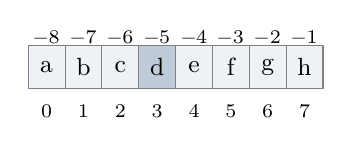
\begin{tikzpicture}[line join=round]
\node[,inner sep=1pt,font=\scriptsize] at (0.306,-0.252) {\ensuremath{-}8};
\filldraw[draw=black!50,fill=Paperblue] (0.072,-0.360) rectangle (0.540,-0.900);
\node[,inner sep=1pt,font=\small] at (0.306,-0.630) {a};
\node[,inner sep=1pt,font=\scriptsize] at (0.306,-1.188) {0};
\node[,inner sep=1pt,font=\scriptsize] at (0.774,-0.252) {\ensuremath{-}7};
\filldraw[draw=black!50,fill=Paperblue] (0.540,-0.360) rectangle (1.008,-0.900);
\node[,inner sep=1pt,font=\small] at (0.774,-0.630) {b};
\node[,inner sep=1pt,font=\scriptsize] at (0.774,-1.188) {1};
\node[,inner sep=1pt,font=\scriptsize] at (1.242,-0.252) {\ensuremath{-}6};
\filldraw[draw=black!50,fill=Paperblue] (1.008,-0.360) rectangle (1.476,-0.900);
\node[,inner sep=1pt,font=\small] at (1.242,-0.630) {c};
\node[,inner sep=1pt,font=\scriptsize] at (1.242,-1.188) {2};
\node[,inner sep=1pt,font=\scriptsize] at (1.710,-0.252) {\ensuremath{-}5};
\filldraw[draw=black!50,fill=FAUblue!25] (1.476,-0.360) rectangle (1.944,-0.900);
\node[,inner sep=1pt,font=\small] at (1.710,-0.630) {d};
\node[,inner sep=1pt,font=\scriptsize] at (1.710,-1.188) {3};
\node[,inner sep=1pt,font=\scriptsize] at (2.178,-0.252) {\ensuremath{-}4};
\filldraw[draw=black!50,fill=Paperblue] (1.944,-0.360) rectangle (2.412,-0.900);
\node[,inner sep=1pt,font=\small] at (2.178,-0.630) {e};
\node[,inner sep=1pt,font=\scriptsize] at (2.178,-1.188) {4};
\node[,inner sep=1pt,font=\scriptsize] at (2.646,-0.252) {\ensuremath{-}3};
\filldraw[draw=black!50,fill=Paperblue] (2.412,-0.360) rectangle (2.880,-0.900);
\node[,inner sep=1pt,font=\small] at (2.646,-0.630) {f};
\node[,inner sep=1pt,font=\scriptsize] at (2.646,-1.188) {5};
\node[,inner sep=1pt,font=\scriptsize] at (3.114,-0.252) {\ensuremath{-}2};
\filldraw[draw=black!50,fill=Paperblue] (2.880,-0.360) rectangle (3.348,-0.900);
\node[,inner sep=1pt,font=\small] at (3.114,-0.630) {g};
\node[,inner sep=1pt,font=\scriptsize] at (3.114,-1.188) {6};
\node[,inner sep=1pt,font=\scriptsize] at (3.582,-0.252) {\ensuremath{-}1};
\filldraw[draw=black!50,fill=Paperblue] (3.348,-0.360) rectangle (3.816,-0.900);
\node[,inner sep=1pt,font=\small] at (3.582,-0.630) {h};
\node[,inner sep=1pt,font=\scriptsize] at (3.582,-1.188) {7};
\end{tikzpicture}\par\smallskip{\small\raggedright \textbf{\texttt{s = "abcdefgh"}.} Index from the left below each box, from the right above it. \texttt{s[3]} and \texttt{s[-5]} name the same character.\par}\end{minipage}
\end{center}

Strings compare with \texttt{==}, \texttt{\ensuremath{<}}, \texttt{\ensuremath{>}} like numbers (§6.6), and they are case sensitive: \texttt{"abc" == "ABC"} is \texttt{False}. Indexing past the end, as in \texttt{"abc"[3]}, raises an error.

\begin{keepsection}
\Needspace{7\baselineskip}
\subsection{Slicing in practice}

With \texttt{s = "abcdefgh"}: \texttt{s[3:6]} is \texttt{"def"} (indices 3, 4, 5); \texttt{s[3:6:2]} is \texttt{"df"}; \texttt{s[::]} is the whole string; \texttt{s[::-1]} is \texttt{"hgfedcba"}, the string reversed; and \texttt{s[4:1:-2]} is \texttt{"ec"}. The lecture prints the reversed string as “hgfedbca”, which is a typo (see the slips list).
\end{keepsection}

\begin{keepsection}
\Needspace{13\baselineskip}
\subsection{Immutability}

\Needspace{10\baselineskip}
\texttt{s[0] = 'y'} fails with an error, because a string object cannot be modified. To get \texttt{"yello"} from \texttt{"hello"}, build a new string and rebind the name: \texttt{s = 'y' + s[1:len(s)]}.

\begin{workedbox}{Worked example \ensuremath{\cdot} s[4:1:-2] with s = "abcdefgh"}
\Needspace{9\baselineskip}
\begin{enumerate}
\item Start at index 4: \texttt{"e"}.
\item Step \ensuremath{-}2 to index 2: \texttt{"c"}.
\item The next index would be 0, which is not before \texttt{stop} = 1 in the backwards direction, so the slice ends.
\item Result \texttt{"ec"}. Check: a negative step walks right to left, so the result must read backwards through the string.
\end{enumerate}
\end{workedbox}

\Needspace{5\baselineskip}
\begin{notebox}\textbf{Trap:} the \texttt{stop} index is never included. \texttt{s[3:6]} has three characters, 6 \ensuremath{-} 3, not four.\end{notebox}

\Needspace{5\baselineskip}
\begin{notebox}\textbf{Near miss:} \texttt{s[len(s)]} looks like “the last character”, but indices end at \texttt{len(s) - 1}, so it is out of bounds and raises an error. Use \texttt{s[-1]}.\end{notebox}

\Needspace{9\baselineskip}
\begin{recallbox}{Recall check \ensuremath{\cdot} answer without looking}
\Needspace{4\baselineskip}
\begin{enumerate}
\item With \texttt{s = "python"}, give \texttt{s[0]}, \texttt{s[-1]} and \texttt{s[1:4]}.
\item Why does \texttt{s[0] = "P"} fail, and what do you write instead?
\end{enumerate}

\nopagebreak[4]{\small\itshape Answers: see “6.4 Strings” under Answers at the end.}
\end{recallbox}
\end{keepsection}
\end{keepsection}

\begin{keepsection}
\Needspace{11\baselineskip}
\section{6.5 Output and input}

\Needspace{8\baselineskip}
A program talks to its user through \texttt{print} and listens through \texttt{input}; the type that \texttt{input} returns is the usual source of errors.

\Needspace{13\baselineskip}
\begin{plainbox}\textbf{In plain words:} \textbf{\texttt{print}} writes values to the console. Give it several values separated by commas and it puts a space between them. \textbf{\texttt{input}} shows a prompt, waits for the user to type something and press Enter, and hands back what was typed, always as a string, even if the user typed digits.\end{plainbox}

\begin{equationcard}{Output and input}
\[ \begin{gathered} \texttt{print(a, b, c)}:\, \text{the}\, \text{values}\, \text{with}\, \text{one}\, \text{space}\, \text{between}\, \text{each} \\ \texttt{text = input("prompt")}:\, \texttt{text}\, \text{is}\, \mathrm{a}\, \texttt{str} \\ \texttt{num = int(input("prompt"))}:\, \text{cast}\, \text{to}\, \text{use}\, \text{it}\, \text{as}\, \mathrm{a}\, \text{number} \end{gathered} \]
{\small \emph{Read it as: “print shows the values separated by spaces; input returns a string, so cast it before arithmetic”.}\par  Joining with \texttt{+} needs every part to be a string already: cast numbers with \texttt{str}.}
\end{equationcard}

\Needspace{13\baselineskip}
The lecture prints the same sentence two ways. \texttt{print("my fav num is", x, ".", "x =", x)} passes five values and prints \texttt{my fav num is 1 . x = 1}, with a space before the full stop. \texttt{print("my fav num is " + x\_str + ". " + "x = " + x\_str)} builds one string from strings and prints \texttt{my fav num is 1. x = 1}, with exactly the spaces you typed.

\begin{workedbox}{Worked example \ensuremath{\cdot} the user types 4}
\Needspace{8\baselineskip}
\begin{enumerate}
\item \texttt{text = input("Type anything... ")} binds \texttt{text} to the string \texttt{"4"}.
\item \texttt{print(5*text)} repeats the string: it prints \texttt{44444}.
\item \texttt{num = int(input("Type a number... "))} with input 4 binds \texttt{num} to the int 4; \texttt{print(5*num)} prints \texttt{20}.
\item Check: the same keystrokes give a string unless you cast, and \texttt{*} on a string repeats it.
\end{enumerate}
\end{workedbox}

\Needspace{6\baselineskip}
\begin{notebox}\textbf{Trap:} \texttt{print("total: " + 3)} raises a \texttt{TypeError}, because \texttt{+} cannot join a string and an int. Write \texttt{print("total:", 3)} or \texttt{"total: " + str(3)}.\end{notebox}

\Needspace{10\baselineskip}
\begin{notebox}\textbf{Near miss:} in the shell, typing \texttt{3+2} shows 5, so it looks as if the expression printed itself; in a script file that line shows nothing. Only \texttt{print} writes to the console from a program.\end{notebox}

\begin{recallbox}{Recall check \ensuremath{\cdot} answer without looking}
\Needspace{4\baselineskip}
\begin{enumerate}
\item What type does \texttt{input} return, and what must you do before using the answer in arithmetic?
\item What does \texttt{print("a", 1, "b")} show?
\end{enumerate}

\nopagebreak[4]{\small\itshape Answers: see “6.5 Output and input” under Answers at the end.}
\end{recallbox}
\end{keepsection}

\begin{keepsection}
\Needspace{10\baselineskip}
\section{6.6 Comparison and logic}

\Needspace{7\baselineskip}
Branches and loops are steered by conditions; a condition is an expression whose value is \texttt{True} or \texttt{False}.

\Needspace{11\baselineskip}
\begin{plainbox}\textbf{In plain words:} a \textbf{comparison} asks a yes-or-no question about two values, such as “is \textit{i} larger than \textit{j}?”, and its answer is a Boolean. The \textbf{logic operators} \texttt{not}, \texttt{and} and \texttt{or} combine Booleans into bigger questions, exactly like NOT, AND and OR in Boolean algebra.\end{plainbox}

\begin{equationcard}{Comparison operators}
\[ \begin{gathered} \texttt{i \ensuremath{>} j}\, \cdot \, \texttt{i \ensuremath{>}= j}\, \cdot \, \texttt{i \ensuremath{<} j}\, \cdot \, \texttt{i \ensuremath{<}= j} \\ \texttt{i == j}:\, \text{equal}\, \cdot \, \texttt{i != j}:\, \text{not}\, \text{equal} \end{gathered} \]
{\small \emph{Read it as: “greater, greater or equal, less, less or equal, equal, not equal”.}\par  They work on ints, floats and strings, and each gives a \texttt{bool}.}
\end{equationcard}

\begin{equationcard}{Logic operators}
\[ \begin{gathered} \texttt{not a}:\, \texttt{True}\, \text{exactly}\, \text{when}\, \texttt{a}\, \text{is}\, \texttt{False} \\ \texttt{a and b}:\, \texttt{True}\, \text{only}\, \text{when}\, \text{both}\, \text{are}\, \texttt{True} \\ \texttt{a or b}:\, \texttt{True}\, \text{when}\, \text{at}\, \text{least}\, \text{one}\, \text{is}\, \texttt{True} \end{gathered} \]
{\small \emph{Read it as: “not a flips a; a and b needs both; a or b needs one or both”.}\par  Python applies \texttt{not} first, then \texttt{and}, then \texttt{or}, all after the comparisons.}
\end{equationcard}

\Needspace{9\baselineskip}
The lecture’s example: with \texttt{set\_time = 15} and \texttt{sleep\_time = 8}, \texttt{print(sleep\_time \ensuremath{>} set\_time)} prints \texttt{False}. In the second example \texttt{derive} is \texttt{True} and \texttt{drink} is \texttt{False}, so \texttt{both = drink and derive} gives \texttt{False}: one operand is \texttt{False}.

\Needspace{12\baselineskip}
Strings compare character by character, using the character codes from Chapter 3. (This follows from the codes; the slides only say strings can be compared.) Every capital letter has a smaller code than every small letter, so \texttt{"Zebra" \ensuremath{<} "apple"} is \texttt{True}, and the digit strings \texttt{"10" \ensuremath{<} "9"} is \texttt{True} because \texttt{"1"} comes before \texttt{"9"}.

\begin{workedbox}{Worked example \ensuremath{\cdot} not 3 \ensuremath{>} 2 or 4 \ensuremath{<} 1}
\Needspace{7\baselineskip}
\begin{enumerate}
\item Comparisons first: \texttt{3 \ensuremath{>} 2} is \texttt{True}, \texttt{4 \ensuremath{<} 1} is \texttt{False}.
\item \texttt{not} before \texttt{or}: \texttt{not True} is \texttt{False}.
\item \texttt{False or False} is \texttt{False}.
\item Check: the only way to get \texttt{True} from \texttt{or} is a \texttt{True} operand, and none is left.
\end{enumerate}
\end{workedbox}

\Needspace{7\baselineskip}
\begin{notebox}\textbf{Trap:} comparing a number with a string of digits does not convert either side. \texttt{5 == "5"} is \texttt{False}; cast first.\end{notebox}

\Needspace{10\baselineskip}
\begin{notebox}\textbf{Near miss:} \texttt{"10" \ensuremath{<} "9"} looks false, since 10 is bigger than 9, but these are strings: they compare character by character, and \texttt{"1"} is before \texttt{"9"}, so it is \texttt{True}. Compare \texttt{int("10") \ensuremath{<} int("9")} for the numbers.\end{notebox}

\begin{recallbox}{Recall check \ensuremath{\cdot} answer without looking}
\Needspace{4\baselineskip}
\begin{enumerate}
\item What is the type of the value of \texttt{3 \ensuremath{<} 4}?
\item For which values of \texttt{a} and \texttt{b} is \texttt{a or b} \texttt{False}?
\end{enumerate}

\nopagebreak[4]{\small\itshape Answers: see “6.6 Comparison and logic” under Answers at the end.}
\end{recallbox}
\end{keepsection}

\begin{keepsection}
\Needspace{10\baselineskip}
\section{6.7 Branching and indentation}

\Needspace{7\baselineskip}
With conditions in hand, a program can choose which block of lines to run.

\Needspace{12\baselineskip}
\begin{plainbox}\textbf{In plain words:} an \textbf{\texttt{if}} statement is a fork in the road: if the condition is true, take this path; otherwise skip it. \textbf{\texttt{elif}} adds more forks, tried in order, and \textbf{\texttt{else}} catches everything left over. Python knows which lines belong to which path by their \textbf{indentation}: the lines of one block are pushed in by the same amount.\end{plainbox}

\begin{equationcard}{The three forms}
\[ \begin{gathered} \texttt{if c:}\, \text{block} \\ \texttt{if c:}\, \text{block}\, \texttt{else:}\, \text{block} \\ \texttt{if c1:}\, \text{block}\, \texttt{elif c2:}\, \text{block}\, \texttt{else:}\, \text{block} \end{gathered} \]
{\small \emph{Read it as: “if c holds, run the block; with elif, try each condition in order; else runs when none held”.}\par  At most one block of an \texttt{if}/\texttt{elif}/\texttt{else} chain runs: the first whose condition is \texttt{True}.}
\end{equationcard}
\begin{tcolorbox}[colback=Paperblue,colframe=Paperblue,boxrule=0pt,arc=0pt,left=7pt,right=7pt,top=5pt,bottom=5pt]\small\sloppy
\noindent\hspace*{0em}\texttt{x = float(input("Enter a number for x: "))}\par
\noindent\hspace*{0em}\texttt{y = float(input("Enter a number for y: "))}\par
\noindent\hspace*{0em}\texttt{if x == y:}\par
\noindent\hspace*{1em}\texttt{print("x and y are equal")}\par
\noindent\hspace*{1em}\texttt{if y != 0:}\par
\noindent\hspace*{3em}\texttt{print("therefore, x / y is", x/y)}\par
\noindent\hspace*{0em}\texttt{elif x \ensuremath{<} y:}\par
\noindent\hspace*{1em}\texttt{print("x is smaller")}\par
\noindent\hspace*{0em}\texttt{else:}\par
\noindent\hspace*{1em}\texttt{print("y is smaller")}\par
\noindent\hspace*{0em}\texttt{print("thanks!")}\par
\end{tcolorbox}

\Needspace{13\baselineskip}
This is the lecture’s program. The two lines under \texttt{if x == y:} form one block; the inner \texttt{if} has its own, deeper block. The last line is not indented, so it runs whichever branch was taken. The condition uses \texttt{==}: writing \texttt{if x = y:} is a syntax error, because \texttt{=} is assignment, not comparison.

\begin{workedbox}{Worked example \ensuremath{\cdot} run the program with x = 0 and y = 0}
\Needspace{8\baselineskip}
\begin{enumerate}
\item \texttt{x == y} is \texttt{True}, so the first block runs and prints \texttt{x and y are equal}.
\item Inside it, \texttt{y != 0} is \texttt{False}, so the division line is skipped: no division by zero happens.
\item The \texttt{elif} and \texttt{else} blocks are skipped because a branch was already taken.
\item The unindented \texttt{print("thanks!")} runs. Output: two lines. Check: the inner \texttt{if} guards the division exactly in the case where it would fail.
\end{enumerate}
\end{workedbox}

\Needspace{7\baselineskip}
\begin{notebox}\textbf{Trap:} moving \texttt{print("thanks!")} four spaces to the right puts it inside the \texttt{else} block, so it would print only when \textit{y} is smaller. In Python, indentation changes meaning.\end{notebox}

\Needspace{6\baselineskip}
\begin{notebox}\textbf{Near miss:} with \texttt{x = 7}, the chain \texttt{if x \ensuremath{>} 5: … elif x \ensuremath{>} 3: …} has two true conditions, so it seems both blocks should run, but only the first true one does. Separate \texttt{if} statements would run both.\end{notebox}

\Needspace{9\baselineskip}
\begin{recallbox}{Recall check \ensuremath{\cdot} answer without looking}
\Needspace{4\baselineskip}
\begin{enumerate}
\item How does Python know where an \texttt{if} block ends?
\item In an \texttt{if}/\texttt{elif}/\texttt{else} chain, how many blocks can run?
\end{enumerate}

\nopagebreak[4]{\small\itshape Answers: see “6.7 Branching and indentation” under Answers at the end.}
\end{recallbox}
\end{keepsection}

\begin{keepsection}
\Needspace{10\baselineskip}
\section{6.8 while and for loops}

\Needspace{7\baselineskip}
Branching runs a block once or not at all; a loop runs it again and again.

\Needspace{12\baselineskip}
\begin{plainbox}\textbf{In plain words:} a \textbf{\texttt{while} loop} keeps repeating its block as long as its condition stays true, checking before every round. A \textbf{\texttt{for} loop} runs its block once for every value in a sequence, putting each value in turn into the \textbf{loop variable}. \textbf{\texttt{range}} makes a sequence of whole numbers to count with.\end{plainbox}

\begin{equationcard}{while}
\[ \begin{gathered} \texttt{while c:}\, \text{block} \end{gathered} \]
{\small \emph{Read it as: “while c is true, run the block, then check c again”.}\par  If \texttt{c} is \texttt{False} at the first check, the block never runs. Something in the block must eventually make \texttt{c} false, or the loop never ends.}
\end{equationcard}

\begin{equationcard}{range}
\[ \begin{gathered} \texttt{range(stop)}:\, 0,\, 1,\, …,\, \texttt{stop}\, -\, 1 \\ \texttt{range(start, stop, step)}:\, \texttt{start},\, \texttt{start}\, +\, \texttt{step},\, …\, \text{while}\, \text{still}\, \text{before}\, \texttt{stop} \end{gathered} \]
{\small \emph{Read it as: “from start, counting up by step, stopping before stop”.}\par  \texttt{start} defaults to 0 and \texttt{step} to 1. \texttt{stop} itself is never produced: \texttt{range(5, 11, 2)} gives 5, 7, 9. With a negative step it counts down and stops before reaching \texttt{stop} from above: \texttt{range(10, 0, -3)} gives 10, 7, 4, 1.}
\end{equationcard}

\Needspace{14\baselineskip}
\begin{center}
\begin{minipage}[t]{0.950\linewidth}\centering
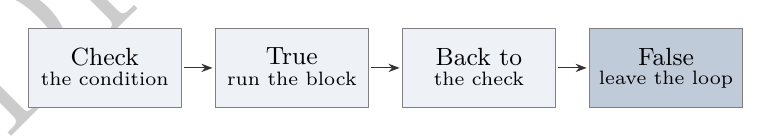
\begin{tikzpicture}[line join=round]
\filldraw[draw=black!50,fill=Paperblue] (0.072,-0.180) rectangle (2.016,-1.188);
\node[,inner sep=1pt,font=\small] at (1.044,-0.540) {Check};
\node[,inner sep=1pt,font=\scriptsize] at (1.044,-0.828) {the condition};
\draw[-{Stealth[length=4pt]},black!80] (2.052,-0.684) -- (2.412,-0.684);
\filldraw[draw=black!50,fill=Paperblue] (2.448,-0.180) rectangle (4.392,-1.188);
\node[,inner sep=1pt,font=\small] at (3.420,-0.540) {True};
\node[,inner sep=1pt,font=\scriptsize] at (3.420,-0.828) {run the block};
\draw[-{Stealth[length=4pt]},black!80] (4.428,-0.684) -- (4.788,-0.684);
\filldraw[draw=black!50,fill=Paperblue] (4.824,-0.180) rectangle (6.768,-1.188);
\node[,inner sep=1pt,font=\small] at (5.796,-0.540) {Back to};
\node[,inner sep=1pt,font=\scriptsize] at (5.796,-0.828) {the check};
\draw[-{Stealth[length=4pt]},black!80] (6.804,-0.684) -- (7.164,-0.684);
\filldraw[draw=black!50,fill=FAUblue!25] (7.200,-0.180) rectangle (9.144,-1.188);
\node[,inner sep=1pt,font=\small] at (8.172,-0.540) {False};
\node[,inner sep=1pt,font=\scriptsize] at (8.172,-0.828) {leave the loop};
\end{tikzpicture}\par\smallskip{\small\raggedright \textbf{A while loop.} The condition is tested before every round, so the last step is reached only when the test fails.\par}\end{minipage}
\end{center}
\begin{tcolorbox}[colback=Paperblue,colframe=Paperblue,boxrule=0pt,arc=0pt,left=7pt,right=7pt,top=5pt,bottom=5pt]\small\sloppy
\noindent\hspace*{0em}\texttt{\# with while: set up, test and update the counter yourself}\par
\noindent\hspace*{0em}\texttt{n = 0}\par
\noindent\hspace*{0em}\texttt{while n \ensuremath{<} 5:}\par
\noindent\hspace*{1em}\texttt{print(n)}\par
\noindent\hspace*{1em}\texttt{n = n+1}\par
\noindent\hspace*{0em}\texttt{}\par
\noindent\hspace*{0em}\texttt{\# with for: range does the counting}\par
\noindent\hspace*{0em}\texttt{for n in range(5):}\par
\noindent\hspace*{1em}\texttt{print(n)}\par
\end{tcolorbox}

\Needspace{12\baselineskip}
Both loops print 0 to 4. The \texttt{for} version is shorter because \texttt{range} sets the start, the step and the end. A \texttt{for} loop is not limited to numbers: it can walk through any sequence, such as the characters of a string (§6.10).

\begin{workedbox}{Worked example \ensuremath{\cdot} the lecture’s two sums}
\Needspace{7\baselineskip}
\begin{enumerate}
\item \texttt{for i in range(7, 10): mysum += i} with \texttt{mysum = 0}: \textit{i} takes 7, 8, 9, so \texttt{mysum} is 24.
\item \texttt{for i in range(5, 11, 2): mysum += i}: \textit{i} takes 5, 7, 9 (11 is not produced, and neither is 10), so \texttt{mysum} is 21.
\item Check by count: \texttt{range(7, 10)} has 10 \ensuremath{-} 7 = 3 values; \texttt{range(5, 11, 2)} has 3 values because the next value would be 11, which is not before \texttt{stop}.
\end{enumerate}
\end{workedbox}

\Needspace{6\baselineskip}
\begin{notebox}\textbf{Trap:} a \texttt{while} loop whose body never changes the condition runs forever. Before you run one, name the line that moves it towards stopping.\end{notebox}

\Needspace{5\baselineskip}
\begin{notebox}\textbf{Near miss:} \texttt{range(1, 5)} looks as if it counts 1 to 5, but it stops before 5: 1, 2, 3, 4. To include 5 write \texttt{range(1, 6)}.\end{notebox}

\Needspace{9\baselineskip}
\begin{recallbox}{Recall check \ensuremath{\cdot} answer without looking}
\Needspace{4\baselineskip}
\begin{enumerate}
\item List the values of \texttt{range(4, 6)} and of \texttt{range(10, 0, -3)}.
\item When does the body of a \texttt{while} loop run zero times?
\end{enumerate}

\nopagebreak[4]{\small\itshape Answers: see “6.8 while and for loops” under Answers at the end.}
\end{recallbox}
\end{keepsection}

\begin{keepsection}
\Needspace{9\baselineskip}
\section{6.9 break and continue}

\Needspace{6\baselineskip}
Sometimes a loop should stop early or skip the rest of one round; two keywords do this.

\Needspace{11\baselineskip}
\begin{plainbox}\textbf{In plain words:} \textbf{\texttt{break}} is an emergency exit: it leaves the loop at once and carries on after it. \textbf{\texttt{continue}} skips the rest of this round only and jumps back to the top of the loop for the next round. Both affect only the innermost loop they sit in.\end{plainbox}

\begin{equationcard}{Jumps inside a loop}
\[ \begin{gathered} \texttt{break}:\, \text{leave}\, \text{the}\, \text{innermost}\, \text{loop}\, \text{now} \\ \texttt{continue}:\, \text{skip}\, \text{the}\, \text{rest}\, \text{of}\, \text{this}\, \text{round},\, \text{start}\, \text{the}\, \text{next} \end{gathered} \]
{\small \emph{Read it as: “break exits the loop; continue skips to the next round”.}\par  The lines after either keyword in the same block do not run in that round. A \texttt{break} in an inner loop leaves the outer loop running.}
\end{equationcard}
\begin{tcolorbox}[colback=Paperblue,colframe=Paperblue,boxrule=0pt,arc=0pt,left=7pt,right=7pt,top=5pt,bottom=5pt]\small\sloppy
\noindent\hspace*{0em}\texttt{mysum = 0}\par
\noindent\hspace*{0em}\texttt{for i in range(5, 11, 2):}\par
\noindent\hspace*{1em}\texttt{mysum += i}\par
\noindent\hspace*{1em}\texttt{if mysum == 5:}\par
\noindent\hspace*{3em}\texttt{break \# or: continue}\par
\noindent\hspace*{1em}\texttt{mysum += 1}\par
\noindent\hspace*{0em}\texttt{print(mysum)}\par
\end{tcolorbox}

\begin{workedbox}{Worked example \ensuremath{\cdot} the lecture’s break and continue programs}
\Needspace{7\baselineskip}
\begin{enumerate}
\item With \texttt{break}: \textit{i} = 5 makes \texttt{mysum} 5, the test is true, and the loop ends. It prints \texttt{5}.
\item With \texttt{continue}, round \textit{i} = 5: \texttt{mysum} becomes 5, the test is true, and \texttt{mysum += 1} is skipped.
\item Round \textit{i} = 7: \texttt{mysum} is 12, the test is false, then 13. Round \textit{i} = 9: 22, then 23.
\item It prints \texttt{23}. Check: \texttt{continue} skipped exactly one \texttt{+= 1}, and 5 + 7 + 9 + 2 = 23.
\end{enumerate}
\end{workedbox}

\Needspace{7\baselineskip}
\begin{notebox}\textbf{Trap:} \texttt{break} in a nested loop exits only the inner one. With \texttt{for i in range(3):} around \texttt{for j in range(4):} and \texttt{if j == 2: break} as the first line of the inner body, the rest of that body runs twice per outer round: 6 times in total.\end{notebox}

\Needspace{5\baselineskip}
\begin{notebox}\textbf{Near miss:} \texttt{continue} sounds like “keep going with the next line”, but it does the opposite: it skips the remaining lines of this round and starts the next round.\end{notebox}

\Needspace{9\baselineskip}
\begin{recallbox}{Recall check \ensuremath{\cdot} answer without looking}
\Needspace{4\baselineskip}
\begin{enumerate}
\item What is the difference between \texttt{break} and \texttt{continue}?
\item After \texttt{for i in range(10):} with \texttt{if i * i \ensuremath{>} 20: break} inside, what is \textit{i}?
\end{enumerate}

\nopagebreak[4]{\small\itshape Answers: see “6.9 break and continue” under Answers at the end.}
\end{recallbox}
\end{keepsection}

\begin{keepsection}
\Needspace{11\baselineskip}
\section{6.10 Choosing a loop and iterating over strings}

\Needspace{8\baselineskip}
Both loops can repeat a block; choosing the right one, and letting \texttt{for} walk a string directly, makes the code shorter and safer.

\Needspace{12\baselineskip}
\begin{plainbox}\textbf{In plain words:} use \textbf{\texttt{for}} when you know in advance how many rounds you need, or you want one round per item; use \textbf{\texttt{while}} when you stop on a condition and cannot say beforehand how many rounds it will take. Any \texttt{for} loop can be rewritten as a \texttt{while} loop, but not always the other way round. Walking straight through the characters with \texttt{for char in s} is called the \textbf{pythonic} way.\end{plainbox}

\begin{equationcard}{Two ways to walk a string}
\[ \begin{gathered} \texttt{for index in range(len(s)):}\, \text{use}\, \texttt{s[index]} \\ \texttt{for char in s:}\, \text{use}\, \texttt{char} \end{gathered} \]
{\small \emph{Read it as: “loop over the positions and look each one up, or loop over the characters themselves”.}\par  Both visit every character once, in order. The second has no index to get wrong.}
\end{equationcard}

\Needspace{10\baselineskip}
\begin{center}\small\begin{tabularx}{\linewidth}{>{\raggedright\arraybackslash}X>{\raggedright\arraybackslash}X>{\raggedright\arraybackslash}X}\toprule
\textbf{} & \textbf{\texttt{for} loop} & \textbf{\texttt{while} loop} \\ \midrule
Number of rounds & Known in advance & Unbounded: until the condition fails \\
End early & \texttt{break} / \texttt{continue} & \texttt{break} / \texttt{continue} \\
Counter & Provided by the loop & Initialise before, update inside \\
Rewrite as the other & Always possible & Not always possible \\
\bottomrule\end{tabularx}\end{center}

\Needspace{13\baselineskip}
The lecture’s cheering program first walks the word with an index (\texttt{i = 0}, \texttt{while i \ensuremath{<} len(word):}, \texttt{char = word[i]}, …, \texttt{i += 1}) and then replaces those three lines with \texttt{for char in word:}. Inside, \texttt{char in an\_letters} tests whether a one-character string occurs in the string of letters that take “an”.

\begin{workedbox}{Worked example \ensuremath{\cdot} rewrite a for loop as a while loop}
\Needspace{8\baselineskip}
\begin{enumerate}
\item Start: \texttt{for n in range(3, 8): print(n)} prints 3 to 7.
\item Initialise the counter before the loop: \texttt{n = 3}.
\item Test it in the condition: \texttt{while n \ensuremath{<} 8:}, because \texttt{range} stops before 8.
\item Update it at the end of the body: \texttt{print(n)} then \texttt{n += 1}. Check: the last value printed is 7, and the loop stops when \textit{n} reaches 8.
\end{enumerate}
\end{workedbox}

\Needspace{6\baselineskip}
\begin{notebox}\textbf{Trap:} forgetting the update line (\texttt{i += 1}) in a \texttt{while} version of a counting loop gives an endless loop; the lecture crosses out exactly these lines when it switches to \texttt{for}.\end{notebox}

\Needspace{12\baselineskip}
\begin{notebox}\textbf{Near miss:} “read numbers until the user types 0” has a clear end, so it seems a \texttt{for} loop could do it, but nobody knows the count in advance: that is a \texttt{while} loop.\end{notebox}

\begin{recallbox}{Recall check \ensuremath{\cdot} answer without looking}
\Needspace{4\baselineskip}
\begin{enumerate}
\item Give one task that needs a \texttt{while} loop and one that suits a \texttt{for} loop.
\item What three pieces must you add when you turn a \texttt{for … in range(…)} loop into a \texttt{while} loop?
\end{enumerate}

\nopagebreak[4]{\small\itshape Answers: see “6.10 Choosing a loop and iterating over strings” under Answers at the end.}
\end{recallbox}
\end{keepsection}

\begin{keepsection}
\Needspace{21\baselineskip}
\section{Formula map and units}

\Needspace{10\baselineskip}
\begin{center}\small\begin{tabularx}{\linewidth}{>{\raggedright\arraybackslash}X>{\raggedright\arraybackslash}X}\toprule
\textbf{Rule} & \textbf{Result type or meaning} \\ \midrule
\texttt{int} op \texttt{int} for \texttt{+ - * // \% **} & \texttt{int} (a negative power gives a float) \\
any \texttt{float} operand & \texttt{float} \\
\texttt{i / j} & always \texttt{float} \\
\texttt{i == j * (i // j) + i \% j} & always \texttt{True} for ints with \textit{j} \ensuremath{\neq} 0 \\
\texttt{int(x)}, \texttt{float(x)}, \texttt{str(x)} & casts; \texttt{int} of a float truncates towards zero \\
comparisons, \texttt{not}, \texttt{and}, \texttt{or} & \texttt{bool} \\
\texttt{input(…)} & always \texttt{str} \\
\texttt{len(s[a:b])} for 0 \ensuremath{\leq} \textit{a} \ensuremath{\leq} \textit{b} \ensuremath{\leq} \texttt{len(s)} & \textit{b} \ensuremath{-} \textit{a} characters \\
\texttt{range(a, b)} & \textit{b} \ensuremath{-} \textit{a} values, from \textit{a} to \textit{b} \ensuremath{-} 1 \\
precedence & \texttt{( )}, then \texttt{**}, then \texttt{* / // \%}, then \texttt{+ -}, then comparisons, \texttt{not}, \texttt{and}, \texttt{or} \\
\bottomrule\end{tabularx}\end{center}

\begin{notebox}\textbf{Check every answer:} state the type as well as the value (2 or 2.0? 5 or "5"?); check that a slice or range has the number of elements the stop rule predicts; and for a loop, check the first round, the last round and the value left in the loop variable afterwards.\end{notebox}
\end{keepsection}

\begin{keepsection}
\Needspace{14\baselineskip}
\section{Derive it cold}

\Needspace{11\baselineskip}
\begin{enumerate}
\item Show that \texttt{i == j * (i // j) + i \% j} for 7 and 2, and for \ensuremath{-}7 and 2. \hfill{\small\color{FAUblue}§6.2}
\item Evaluate \texttt{2 + 3 * 4 ** 2 // 5} step by step, naming the precedence rule at each step. \hfill{\small\color{FAUblue}§6.2}
\item Trace the four lines \texttt{pi}, \texttt{radius}, \texttt{area}, \texttt{radius = radius+1} and explain why \texttt{area} does not change. \hfill{\small\color{FAUblue}§6.3}
\item Work out \texttt{s[4:1:-2]} and \texttt{s[::-1]} for \texttt{s = "abcdefgh"} index by index. \hfill{\small\color{FAUblue}§6.4}
\item Trace the lecture’s \texttt{break} and \texttt{continue} programs to 5 and 23. \hfill{\small\color{FAUblue}§6.9}
\item Rewrite \texttt{for n in range(3, 8)} as a \texttt{while} loop and name the three pieces you added. \hfill{\small\color{FAUblue}§6.10}
\end{enumerate}
\end{keepsection}

\begin{keepsection}
\Needspace{14\baselineskip}
\section{Explain it}

\Needspace{11\baselineskip}
\begin{enumerate}
\item Why does Python need an interpreter at all, when the processor already runs programs?
\item Why is \texttt{radius = radius + 1} not a contradiction?
\item Why does \texttt{input} return a string even when the user types digits?
\item Why can an \texttt{if}/\texttt{elif} chain behave differently from the same conditions written as separate \texttt{if} statements?
\item When must you use a \texttt{while} loop instead of a \texttt{for} loop?
\item Why is \texttt{for char in s} safer than looping over \texttt{range(len(s))}?
\end{enumerate}

\nopagebreak[4]{\small\itshape Answers: see “Explain it” under Answers at the end.}
\end{keepsection}

\clearpage

\begin{keepsection}
\Needspace{11\baselineskip}
\section{Mixed practice}

\Needspace{8\baselineskip}
Try all 24 problems before opening the answers. The order mixes every section on purpose, so you have to choose the method yourself. Predict each output on paper, then check it in a Python shell.

\begin{enumerate}
\item Give the value and type of \texttt{9 / 3}.
\item With \texttt{s = "python"}, evaluate \texttt{s[1]}, \texttt{s[-2]} and \texttt{s[1:4]}.
\item What does this print? \texttt{x = 5}, then \texttt{x = x * 2 + 1}, then \texttt{print(x)}.
\item List the values of \texttt{range(2, 11, 3)}.
\item Give the value and type of \texttt{int(-2.7)}.
\item Evaluate \texttt{not 1 \ensuremath{>}= 2 and 5 != 5}.
\item Starting from \texttt{n = 10}, the loop \texttt{while n \ensuremath{>} 1: n = n // 2} runs. How many rounds does it make, and what is \textit{n} at the end?
\item A chain prints \texttt{"pos"} under \texttt{if x \ensuremath{>} 0}, \texttt{"zero"} under \texttt{elif x == 0} and \texttt{"neg"} under \texttt{else}. What does it print for \textit{x} = 0?
\item The user types 4 at \texttt{num = input("n: ")}. What does \texttt{print(num * 3)} show?
\item Evaluate \texttt{3 + 2 ** 3 * 4 // 6}, then \texttt{(3 + 2) ** 3 * 4 // 6}. What changes?
\item After \texttt{for i in range(10):} with the body \texttt{if i * i * i \ensuremath{>} 50: break}, what is the value of \textit{i}?
\item Why does \texttt{s[0] = "J"} fail for \texttt{s = "hello"}, and how do you make \texttt{"Jello"}?
\item What is \texttt{total} after \texttt{total = 0} and \texttt{for k in range(1, 6): total += k}?
\item A program should read numbers until the user types 0. Which loop do you use, and why?
\item What do \texttt{print("total:", 3, "items")} and \texttt{print("total:" + 3)} do?
\item Evaluate \texttt{7 \% 3}, \texttt{-7 \% 3} and \texttt{7 // 2.0}.
\item What is \texttt{count} after \texttt{count = 0} and \texttt{for ch in "a-b-c":} with the body \texttt{if ch == "-": continue} then \texttt{count += 1}?
\item In the lecture’s \texttt{x}/\texttt{y} program (§6.7), the user enters 3 and 3. List every line that is printed.
\item Is \texttt{"apple" \ensuremath{<} "Apple"} true or false? Explain.
\item Rewrite \texttt{for n in range(2, 12, 3): print(n)} as a \texttt{while} loop.
\item After \texttt{radius = 2}, \texttt{area = 3 * radius ** 2}, \texttt{radius = 5}, what is \texttt{area}?
\item With \texttt{s = "abcdefgh"}, evaluate \texttt{s[::-1]} and \texttt{s[6:2:-2]}.
\item You save three lines of Python in a file and run it. Is it compiled to machine code first, as a C program would be? What happens instead?
\item Rewrite \texttt{i = 0} / \texttt{while i \ensuremath{<} len(word):} / \texttt{char = word[i]} / … / \texttt{i += 1} in the pythonic form, and say how many times the body runs for \texttt{word = "loop"}.
\end{enumerate}

\nopagebreak[4]{\small\itshape Answers: see “Mixed practice” under Answers at the end.}
\end{keepsection}

\begin{keepsection}
\section{Exam-style problems}

\begin{keepsection}
\Needspace{4\baselineskip}
\subsection{1 \ensuremath{\cdot} A score averager \ensuremath{\cdot} 20 minutes}
\begin{tcolorbox}[colback=Paperblue,colframe=Paperblue,boxrule=0pt,arc=0pt,left=7pt,right=7pt,top=5pt,bottom=5pt]\small\sloppy
\noindent\hspace*{0em}\texttt{total = 0}\par
\noindent\hspace*{0em}\texttt{count = 0}\par
\noindent\hspace*{0em}\texttt{while True:}\par
\noindent\hspace*{1em}\texttt{entry = input("score (q to stop): ")}\par
\noindent\hspace*{1em}\texttt{if entry == "q":}\par
\noindent\hspace*{3em}\texttt{break}\par
\noindent\hspace*{1em}\texttt{score = int(entry)}\par
\noindent\hspace*{1em}\texttt{if score \ensuremath{<} 0 or score \ensuremath{>} 100:}\par
\noindent\hspace*{3em}\texttt{continue}\par
\noindent\hspace*{1em}\texttt{total += score}\par
\noindent\hspace*{1em}\texttt{count += 1}\par
\noindent\hspace*{0em}\texttt{print(count, total / count)}\par
\end{tcolorbox}

\Needspace{7\baselineskip}
\begin{enumerate}
\item Why does the program need \texttt{int(entry)}, and why must the test for \texttt{"q"} come before it?
\item The user enters 80, 105, 70 and then q. Trace \texttt{total} and \texttt{count} and give the printed line.
\item What happens if the user types q at the first prompt? Change the last line to avoid it.
\item Why is this a \texttt{while} loop and not a \texttt{for} loop, and how does it ever end?
\end{enumerate}

\nopagebreak[4]{\small\itshape Answers: see “Exam-style problems” under Answers at the end.}
\end{keepsection}

\begin{keepsection}
\Needspace{4\baselineskip}
\subsection{2 \ensuremath{\cdot} A palindrome check \ensuremath{\cdot} 20 minutes}
\begin{tcolorbox}[colback=Paperblue,colframe=Paperblue,boxrule=0pt,arc=0pt,left=7pt,right=7pt,top=5pt,bottom=5pt]\small\sloppy
\noindent\hspace*{0em}\texttt{word = "racecar"}\par
\noindent\hspace*{0em}\texttt{i = 0}\par
\noindent\hspace*{0em}\texttt{same = True}\par
\noindent\hspace*{0em}\texttt{while i \ensuremath{<} len(word) // 2:}\par
\noindent\hspace*{1em}\texttt{if word[i] != word[-1 - i]:}\par
\noindent\hspace*{3em}\texttt{same = False}\par
\noindent\hspace*{3em}\texttt{break}\par
\noindent\hspace*{1em}\texttt{i += 1}\par
\noindent\hspace*{0em}\texttt{print(same)}\par
\end{tcolorbox}

\Needspace{8\baselineskip}
\begin{enumerate}
\item How many rounds can the loop make for \texttt{"racecar"}, and which pairs of characters does it compare?
\item Trace the program for \texttt{word = "rocket"}: what are \textit{i} and \texttt{same} at the end?
\item Give a one-line expression with a slice that has the same value as \texttt{same}.
\item Rewrite the loop as a \texttt{for} loop over \texttt{range}.
\end{enumerate}

\nopagebreak[4]{\small\itshape Answers: see “Exam-style problems” under Answers at the end.}
\end{keepsection}
\end{keepsection}

\begin{keepsection}
\Needspace{25\baselineskip}
\section{Slips in the notes}

\Needspace{22\baselineskip}
Each item was checked against the rendered slides and against Python 3. Slide numbers refer to “06\_branching\_and\_iterations.pdf”.

\Needspace{19\baselineskip}
\begin{itemize}
\item \textbf{Slide 9, floor division.} \texttt{i//j} is described as returning the quotient as an integer. That holds only for two int operands; with a float operand the floor is a float, so \texttt{7.0 // 2} is \texttt{3.0} (§6.2).
\item \textbf{Slide 10, precedence.} The list shows \texttt{**}, then \texttt{*}, then \texttt{/} on separate rows, which reads as if \texttt{*} ranks above \texttt{/}. In Python, \texttt{*}, \texttt{/}, \texttt{//} and \texttt{\%} share one level and are evaluated left to right, so \texttt{8 / 2 * 4} is \texttt{16.0}. This guide follows Python (§6.2).
\item \textbf{Slide 11, variable name.} \texttt{pi\_approx. = 22/7} is a syntax error: a name cannot contain a dot. It probably means \texttt{pi\_approx = 22/7} (§6.3).
\item \textbf{Slide 16, quotation marks.} The string examples are typeset with curly quotes (“Joe”). Typed into Python, curly quotes are a syntax error; use straight quotes, \texttt{"Joe"} or \texttt{'Joe'}, as this guide does (§6.4).
\item \textbf{Slide 28, range.} “Loop until value is stop \ensuremath{-} 1” is true only for step 1. With \texttt{range(5, 11, 2)} on the same slide, the last value is 9, not 10; the rule is “stop before reaching \texttt{stop}” (§6.8).
\item \textbf{Slide 36, reversed string.} The reversed string \texttt{s[::-1]} is printed as “hgfedbca”; for \texttt{"abcdefgh"} Python gives \texttt{"hgfedcba"}. The slide’s equivalent slice \texttt{s[-1:-(len(s)+1):-1]} is correct (§6.4).
\end{itemize}
\end{keepsection}

\begin{keepsection}
\Needspace{10\baselineskip}
\section{Self-check}

\Needspace{7\baselineskip}
These are the chapter’s learning goals. Tick a skill only in a later session, at least one day after studying, when you can show it without notes.

\begin{itemize}
\item $\mdlgwhtsquare$\ Explain source code, compilers and interpreters, and how Python runs a file. (23)
\item $\mdlgwhtsquare$\ Name the scalar types and cast between them, including truncation. (1, 5)
\item $\mdlgwhtsquare$\ Evaluate \texttt{/}, \texttt{//}, \texttt{\%} and \texttt{**} with the right result type. (1, 10, 16)
\item $\mdlgwhtsquare$\ Apply operator precedence and left-to-right evaluation. (6, 10)
\item $\mdlgwhtsquare$\ Trace assignment and rebinding with a trace table. (3, 21)
\item $\mdlgwhtsquare$\ Index and slice strings, including negative indices and steps. (2, 22)
\item $\mdlgwhtsquare$\ Explain string immutability and build a changed copy. (12)
\item $\mdlgwhtsquare$\ Use \texttt{print} and \texttt{input}, and cast input before arithmetic. (9, 15)
\item $\mdlgwhtsquare$\ Evaluate comparisons and \texttt{not}, \texttt{and}, \texttt{or}, on numbers and strings. (6, 19)
\item $\mdlgwhtsquare$\ Trace \texttt{if}/\texttt{elif}/\texttt{else} chains and nested blocks by indentation. (8, 18)
\item $\mdlgwhtsquare$\ Trace \texttt{while} and \texttt{for} loops and list the values of \texttt{range}. (4, 7, 13)
\item $\mdlgwhtsquare$\ Predict the effect of \texttt{break} and \texttt{continue}, also in nested loops. (11, 17)
\item $\mdlgwhtsquare$\ Choose between \texttt{for} and \texttt{while} and convert one into the other. (14, 20, 24)
\item $\mdlgwhtsquare$\ Rebuild every item in the derivation list on blank paper.
\item $\mdlgwhtsquare$\ Complete both exam-style problems in 20 minutes each.
\end{itemize}
\end{keepsection}


\clearpage
\section{Answers}
\begin{keepsection}\subsection{Start from memory}

\Needspace{8\baselineskip}
\begin{enumerate}
\item \texttt{float}: \texttt{/} always gives a float, here \texttt{1.0}. \hfill{\small\color{FAUblue}§6.2}
\item \texttt{"c"}, the last character. \hfill{\small\color{FAUblue}§6.4}
\item \texttt{=} binds a name to a value; \texttt{==} tests two values for equality and gives a Boolean. \hfill{\small\color{FAUblue}§6.3, §6.6}
\item 0, 1, 2, 3, 4: it starts at 0 and stops before 5. \hfill{\small\color{FAUblue}§6.8}
\item It leaves only the innermost loop; the outer loop carries on. \hfill{\small\color{FAUblue}§6.9}
\end{enumerate}

\end{keepsection}
\begin{keepsection}\subsection{6.1 Programs, Python, objects and types}

\Needspace{6\baselineskip}
\begin{enumerate}
\item The processor runs only its native machine instructions. Source code is human-readable text, so it must be translated (compiler) or read and run step by step (interpreter).
\item \texttt{int}: 5; \texttt{float}: 3.27; \texttt{bool}: \texttt{True}; \texttt{NoneType}: \texttt{None}.
\item \texttt{-2}: the fractional part is cut off.
\end{enumerate}

\end{keepsection}
\begin{keepsection}\subsection{6.2 Expressions and operators}

\Needspace{5\baselineskip}
\begin{enumerate}
\item \texttt{3} (int) and \texttt{3.5} (float).
\item 512: \texttt{**} groups from the right, so it is 2\textsuperscript{9}, not 8\textsuperscript{2} = 64.
\item 2, because 17 = 5 \ensuremath{\cdot} 3 + 2.
\end{enumerate}

\end{keepsection}
\begin{keepsection}\subsection{6.3 Variables and assignment}

\Needspace{6\baselineskip}
\begin{enumerate}
\item The right side is evaluated using the current value of \texttt{count}; then \texttt{count} is rebound to the result.
\item The name can be reused instead of repeating the value, and the code is easier to change later, because the value is set in one place.
\end{enumerate}

\end{keepsection}
\begin{keepsection}\subsection{6.4 Strings}

\Needspace{4\baselineskip}
\begin{enumerate}
\item \texttt{"p"}, \texttt{"n"}, \texttt{"yth"}.
\item Strings are immutable. Build a new string and rebind: \texttt{s = "P" + s[1:]}.
\end{enumerate}

\end{keepsection}
\begin{keepsection}\subsection{6.5 Output and input}

\Needspace{4\baselineskip}
\begin{enumerate}
\item Always a string; cast it, for example with \texttt{int(…)} or \texttt{float(…)}.
\item \texttt{a 1 b}: the values separated by single spaces.
\end{enumerate}

\end{keepsection}
\begin{keepsection}\subsection{6.6 Comparison and logic}

\Needspace{4\baselineskip}
\begin{enumerate}
\item \texttt{bool}; the value is \texttt{True}.
\item Only when both are \texttt{False}.
\end{enumerate}

\end{keepsection}
\begin{keepsection}\subsection{6.7 Branching and indentation}

\Needspace{4\baselineskip}
\begin{enumerate}
\item By indentation: the block ends at the first following line that is indented less.
\item Exactly one if there is an \texttt{else}; at most one without it.
\end{enumerate}

\end{keepsection}
\begin{keepsection}\subsection{6.8 while and for loops}

\Needspace{4\baselineskip}
\begin{enumerate}
\item 4, 5; and 10, 7, 4, 1.
\item When the condition is already \texttt{False} at the first check.
\end{enumerate}

\end{keepsection}
\begin{keepsection}\subsection{6.9 break and continue}

\Needspace{5\baselineskip}
\begin{enumerate}
\item \texttt{break} leaves the loop entirely; \texttt{continue} ends only the current round and goes on with the next.
\item 5, the first value with 5 \ensuremath{\cdot} 5 = 25 \ensuremath{>} 20.
\end{enumerate}

\end{keepsection}
\begin{keepsection}\subsection{6.10 Choosing a loop and iterating over strings}

\Needspace{6\baselineskip}
\begin{enumerate}
\item \texttt{while}: keep asking for a password until it is correct. \texttt{for}: print each character of a word, or sum the numbers 1 to 100.
\item Initialise the counter before the loop, test it in the condition, and update it inside the body.
\end{enumerate}

\end{keepsection}
\begin{keepsection}\subsection{Explain it}

\Needspace{16\baselineskip}
\begin{enumerate}
\item The processor runs only its own machine instructions. Python source code is text, so something has to read it and carry out each line; that is the interpreter. \hfill{\small\color{FAUblue}§6.1}
\item \texttt{=} is assignment, not equality. The right side is evaluated with the old value, and then the name is rebound to the new one. \hfill{\small\color{FAUblue}§6.3}
\item The keyboard delivers characters, and Python cannot know whether you mean the text “42” or the number 42. It hands you the text and leaves the cast to you. \hfill{\small\color{FAUblue}§6.5}
\item A chain runs only the first block whose condition is true and skips the rest. Separate \texttt{if} statements test every condition, so several blocks can run. \hfill{\small\color{FAUblue}§6.7}
\item When the number of rounds is not known in advance, for example when you repeat until a user enters a valid value. A \texttt{for} loop needs its sequence up front. \hfill{\small\color{FAUblue}§6.10}
\item It hands you each character directly, so there is no index to start, update or push past the end. Fewer lines means fewer places for an off-by-one error. \hfill{\small\color{FAUblue}§6.10}
\end{enumerate}

\end{keepsection}
\begin{keepsection}\subsection{Mixed practice}

\begin{enumerate}
\item \texttt{3.0}, a \texttt{float}: \texttt{/} always returns a float, even for an exact division. \hfill{\small\color{FAUblue}§6.2}
\item \texttt{"y"}, \texttt{"o"}, \texttt{"yth"} (indices 1, 2, 3; index 4 is excluded). \hfill{\small\color{FAUblue}§6.4}
\item \texttt{11}: the right side uses the old value 5, so 5 \ensuremath{\cdot} 2 + 1 = 11, then \textit{x} is rebound. \hfill{\small\color{FAUblue}§6.3}
\item 2, 5, 8; the next value, 11, is not before \texttt{stop} = 11. \hfill{\small\color{FAUblue}§6.8}
\item \texttt{-2}, an \texttt{int}: casting cuts the fractional part off towards zero; it does not round down to \ensuremath{-}3. \hfill{\small\color{FAUblue}§6.1}
\item \texttt{False}: \texttt{1 \ensuremath{>}= 2} is \texttt{False}, \texttt{not False} is \texttt{True}, \texttt{5 != 5} is \texttt{False}, and \texttt{True and False} is \texttt{False}. \hfill{\small\color{FAUblue}§6.6}
\item Three rounds: 10 \ensuremath{\to} 5 \ensuremath{\to} 2 \ensuremath{\to} 1. Then \texttt{1 \ensuremath{>} 1} is \texttt{False} and the loop ends with \textit{n} = 1. \hfill{\small\color{FAUblue}§6.8}
\item \texttt{zero}: the first condition is false, the \texttt{elif} condition is true, and the \texttt{else} block is skipped. \hfill{\small\color{FAUblue}§6.7}
\item \texttt{444}: \texttt{num} is the string \texttt{"4"}, and \texttt{*} repeats a string. \hfill{\small\color{FAUblue}§6.5}
\item 8 for the first: 2\textsuperscript{3} = 8, then 8 \ensuremath{\cdot} 4 = 32, then 32 // 6 = 5, then 3 + 5 = 8. With brackets the addition goes first: 5\textsuperscript{3} = 125, 125 \ensuremath{\cdot} 4 = 500, 500 // 6 = 83. \hfill{\small\color{FAUblue}§6.2}
\item 4: for \textit{i} = 0 to 3 the cube is at most 27; at \textit{i} = 4, 64 \ensuremath{>} 50 and \texttt{break} leaves the loop with \textit{i} still 4. \hfill{\small\color{FAUblue}§6.9}
\item Strings are immutable, so a character cannot be assigned. Build a new string: \texttt{s = "J" + s[1:]}. \hfill{\small\color{FAUblue}§6.4}
\item 15: \textit{k} takes 1, 2, 3, 4, 5, and 1 + 2 + 3 + 4 + 5 = 15. \hfill{\small\color{FAUblue}§6.8}
\item A \texttt{while} loop: the number of rounds is not known in advance; the loop stops on a condition (the value read is 0). \hfill{\small\color{FAUblue}§6.10}
\item The first prints \texttt{total: 3 items}, with spaces between the values. The second raises a \texttt{TypeError}: \texttt{+} cannot join a string and an int. \hfill{\small\color{FAUblue}§6.5}
\item 1, 2 and 3.0. For \ensuremath{-}7: \ensuremath{-}7 // 3 is \ensuremath{-}3 (rounded down), and \ensuremath{-}7 \ensuremath{-} 3 \ensuremath{\cdot} (\ensuremath{-}3) = 2. The float operand makes the last result a float. \hfill{\small\color{FAUblue}§6.2}
\item 3: the two \texttt{"-"} characters hit \texttt{continue}, which skips \texttt{count += 1}; the three letters are counted. \hfill{\small\color{FAUblue}§6.9}
\item \texttt{x and y are equal}, then \texttt{therefore, x / y is 1.0}, then \texttt{thanks!}. \hfill{\small\color{FAUblue}§6.7}
\item False. Strings compare by character codes, and every capital letter comes before every small letter, so \texttt{"Apple" \ensuremath{<} "apple"} is the true one. \hfill{\small\color{FAUblue}§6.6}
\item \texttt{n = 2}, then \texttt{while n \ensuremath{<} 12:} with the body \texttt{print(n)} and \texttt{n += 3}; it prints 2, 5, 8, 11. Initialise, test, update by the step. \hfill{\small\color{FAUblue}§6.10}
\item 12: \texttt{area} was computed with \texttt{radius} = 2, and rebinding \texttt{radius} later does not recompute it. \hfill{\small\color{FAUblue}§6.3}
\item \texttt{"hgfedcba"} and \texttt{"ge"} (indices 6 and 4; index 2 is the stop and is excluded). \hfill{\small\color{FAUblue}§6.4}
\item No. Python is an interpreted language: the interpreter reads the file and carries out its commands, without producing a separate machine-code program you run afterwards. \hfill{\small\color{FAUblue}§6.1}
\item \texttt{for char in word:} followed by the same body, without the index lines. The body runs 4 times, once per character of \texttt{"loop"}. \hfill{\small\color{FAUblue}§6.10}
\end{enumerate}

\end{keepsection}
\begin{keepsection}\subsection{Exam-style problems}

\Needspace{11\baselineskip}
\begin{enumerate}
\item \texttt{input} returns a string, so the score must be cast before it is compared with numbers or added. \texttt{int("q")} would raise an error, so the stop test has to run on the raw string first. \hfill{\small\color{FAUblue}§6.5}
\item 80: total 80, count 1. 105: the range test is true, \texttt{continue} skips the update. 70: total 150, count 2. q: \texttt{break}. The program prints \texttt{2 75.0} (a float, because of \texttt{/}). \hfill{\small\color{FAUblue}§6.9, §6.2}
\item \texttt{count} is 0, so \texttt{total / count} divides by zero and the program stops with an error. Guard it: \texttt{if count \ensuremath{>} 0: print(count, total / count)} and \texttt{else: print("no scores")}. \hfill{\small\color{FAUblue}§6.7}
\item Nobody knows in advance how many scores will be entered; the loop stops on a condition, the input q. \texttt{while True} never fails its test, so the only way out is the \texttt{break}. \hfill{\small\color{FAUblue}§6.10, §6.8}
\end{enumerate}

\end{keepsection}
\begin{keepsection}\subsection{Exam-style problems}

\Needspace{11\baselineskip}
\begin{enumerate}
\item \texttt{len("racecar") // 2} is 7 // 2 = 3, so at most three rounds: \texttt{word[0]} with \texttt{word[-1]} (r, r), \texttt{word[1]} with \texttt{word[-2]} (a, a), \texttt{word[2]} with \texttt{word[-3]} (c, c). The middle e needs no partner. All match, so it prints \texttt{True}. \hfill{\small\color{FAUblue}§6.4, §6.8}
\item 6 // 2 = 3 possible rounds. At \textit{i} = 0, r and t differ: \texttt{same} becomes \texttt{False} and \texttt{break} leaves the loop before \texttt{i += 1}, so \textit{i} = 0 and \texttt{same} = \texttt{False}. \hfill{\small\color{FAUblue}§6.9}
\item \texttt{word == word[::-1]}: the word equals its reverse. \hfill{\small\color{FAUblue}§6.4}
\item \texttt{same = True}, then \texttt{for i in range(len(word) // 2):} with the same \texttt{if} and \texttt{break}, and no \texttt{i = 0} or \texttt{i += 1}, because \texttt{range} does the counting. \hfill{\small\color{FAUblue}§6.10}
\end{enumerate}

\end{keepsection}

\vfill{\small Personal study guide based on the supplied “06\_branching\_and\_iterations.pdf” (40 slides, lecture dated 29 April 2024; the slides credit MIT OpenCourseWare 6.0001), written in my own words; no lecture pages or figures are reproduced. Not an official FAU publication; check course details against the current notes. Made by \textbf{Thanate Amornjiraporn (Focus)}.}

\end{document}
